\documentclass[notes]{subfiles}
\begin{document}
	\addcontentsline{toc}{section}{5.2 - The Definite Integral}
	\refstepcounter{section}
	\fancyhead[RO,LE]{\bfseries \nameref{cs52}} 
	\fancyhead[LO,RE]{\bfseries \small \currentname}
	\fancyfoot[C]{{}}
	\fancyfoot[LO,RE]{\large \thepage}	%Footer on Right \thepage is pagenumber
	\fancyfoot[RO,LE]{\large Chapter 5.2}
	
\section*{The Definite Integral}\label{cs52}
	\subsection*{Before Class}
	\subsubsection*{Definition}
		\begin{defn}[Definite Integral]
			Let \(f\) be a function defined for \(a\leq x\leq b\), and divide \([a,b]\) into \(n\) subintervals of width \(\Delta x = \dfrac{b-a}{n}\).  Let 
				\[a=x_0,x_1,x_2,...,x_{n-1},x_n=b\]
			be the endpoints of these subintervals, and let \(x_i^*\) be any sample points in these subintervals, so that \(x_i^*\) lies in the \(i\)th subinterval \([x_{i-1},x_i]\).  Then, the \textbf{definite integral of f from a to b} is given by
					\vspace{.75in}\\
				
			provided that this limit exists and gives the same value for all possible choices of sample points.  If it does exist, we say that \(f\) is \textbf{integrable} on \([a,b]\).\\ \\ \\
			
			The sum 	\blank{2.5} is called a \textbf{Riemann sum}.  		
		\end{defn}
		
		\begin{rmk}[Terminology]
			Given the definite integral \(\ds \int_a^b f(x)\, dx\), we have some terminology:\\ \\
				\begin{itemize}
				\setlength\itemsep{30pt}
					\item $a$ is called the \blank{5}
					\item $b$ is called the \blank{5}
					\item $\ds \int$ is called an \blank{3}
					\item We use $dx$ to denote an \blank{4}
				\end{itemize}
		\end{rmk}
			\newpage
			
		\begin{rmk}[Two Important Integral Facts]
			\begin{itemize}
				\setlength\itemsep{25pt}
					\item If \(f\) is continuous on \([a,b]\), or if \(f\) has \blank{3.6},\vspace{20pt} then \blank{5.5}.			
						
					\item If \(f\) is integrable on \([a,b]\), then\vspace{25pt}
			\end{itemize}
		\end{rmk}
		
		\begin{rmk}[Interpretation of the Integral]
			The definite integral $\ds \int_a^b f(x)\, dx$ can be interpreted as\vspace{5pt}
				\begin{itemize}
				\setlength\itemsep{30pt}
					\item The \emph{total} area between the $f(x)$ and the $x-$axis if \blank{2.5}
					\item The \emph{net} area between $f(x)$ and the $x-$axis if \blank{2.7}\vspace{20pt} \blank{4}
				\end{itemize}
			
		\end{rmk}
		Here are some pictures to help with the interpretations:
			\vs{1}

			\newpage
			
		\begin{ex}
			Express \(\ds \lim_{n\to \infty} \sum_{i = 1}^n \lrpar{x_i^3 - 2x_i^2 + 1 - x_i\cos(x_i)}\Delta x\) as an integral.  Use proper notation.
		\end{ex}
			\vs{1}
			
		\begin{ex}
			Use the definition of the definite integral to show that \(\ds \int_2^4 x\, dx = 6\).
		\end{ex}
			\vs{3}
			\newpage

	\subsubsection*{Pre Class Practice}			
		\begin{ex}
			The shaded area on the graphs of \(\sin x\) and \(\cos x\) are both exactly 1.  
			\begin{center}
				\begin{tikzpicture}
					\begin{axis}[
						width = .5\textwidth,
						every tick label/.append style={font=\scriptsize},
						axis x line = middle,
						axis y line = middle,
						grid = both,
						grid style={line width=.1pt, draw=gray!10},
						major grid style={line width=.2pt,draw=gray!50},
						minor grid style={line width=.2pt, draw=gray!40},
			    			every axis y label/.style={at={(ticklabel cs:1.15)}},
			    			%ytick = {-4, -2, -3, -1, 1, 2, 3, 4},
			    			ymin = -1, ymax = 1,
						y label style={at={(axis description cs:.5,1.15)},anchor=north},
			    			ylabel = {$\sin x$},
		    				every axis x label/.style= {at ={(ticklabel cs:1)}},
		    				xtick = {-7.85, -6.28, -4.71, -3.14,- 1.57,  0, 1.57, 3.14, 4.71, 6.28, 7.85},
		    				x label style={at={(axis description cs:1.1,.5)},anchor=east},
		    				xticklabels = {$-\dfrac{5\pi}{2}$, $-2\pi$, $-\dfrac{3\pi}{2}$, $-\pi$, $-\dfrac{\pi}{2}$,0,$\dfrac{\pi}{2}$, $\pi$, $\dfrac{3\pi}{2}$, $2\pi$, $\dfrac{5\pi}{2}$},
		    				xlabel = {$x$},
		    				xmin = -10, xmax = 10
		    				%minor y tick num = 2,
					]
					
					\addplot[thick,smooth, samples = 100, domain = -10:10, name path = A] {sin(deg(x))};
					\addplot[draw = none, name path = B, domain = 0:1.57] {0};
					\addplot[gray] fill between[of = A and B, soft clip = {domain = 0:1.57}];
					\end{axis}
				\end{tikzpicture}
				\begin{tikzpicture}
					\begin{axis}[
						width = .5\textwidth,
						every tick label/.append style={font=\scriptsize},
						axis x line = middle,
						axis y line = middle,
						grid = both,
						grid style={line width=.1pt, draw=gray!10},
						major grid style={line width=.2pt,draw=gray!50},
						minor grid style={line width=.2pt, draw=gray!40},
			    			every axis y label/.style={at={(ticklabel cs:1.15)}},
			    			%ytick = {-4, -2, -3, -1, 1, 2, 3, 4},
			    			ymin = -1, ymax = 1,
						y label style={at={(axis description cs:.5,1.15)},anchor=north},
			    			ylabel = {$\cos x$},
		    				every axis x label/.style= {at ={(ticklabel cs:1)}},
		    				xtick = {-7.85, -6.28, -4.71, -3.14,- 1.57,  0, 1.57, 3.14, 4.71, 6.28, 7.85},
		    				x label style={at={(axis description cs:1.1,.5)},anchor=east},
		    				xticklabels = {$-\dfrac{5\pi}{2}$, $-2\pi$, $-\dfrac{3\pi}{2}$, $-\pi$, $-\dfrac{\pi}{2}$,0,$\dfrac{\pi}{2}$, $\pi$, $\dfrac{3\pi}{2}$, $2\pi$, $\dfrac{5\pi}{2}$},
		    				xlabel = {$x$},
		    				xmin = -10, xmax = 10
		    				%minor y tick num = 2,
					]
					
					\addplot[thick,smooth, samples = 100, domain = -10:10, name path = A] {cos(deg(x))};
					\addplot[draw = none, name path = B, domain = 0:1.57] {0};
					\addplot[gray] fill between[of = A and B, soft clip = {domain = 0:1.57}];
					\end{axis}
				\end{tikzpicture}
			\end{center}
			\begin{enumerate}[(a)]
				\item Determine the \emph{net area} of \(\sin x\) on the interval \([0,2\pi]\).
					\vs{1}
					
				\item Determine the \emph{total area} of \(\sin x\) on the interval \([0,2\pi]\).
					\vs{1}
					
				\item Determine the \emph{net area} of \(\cos x\) on the interval \(\left[-\dfrac{3\pi}{2}, \pi\right]\).
					\vs{1}
					
				\item Determine the \emph{total area} of \(\cos x\) on the interval \(\left[-\dfrac{3\pi}{2}, \pi\right]\).
					\vs{1}
					
				\item Determine the \emph{net area} of \(\sin x\) on the intervals \(\left[-\dfrac{\pi}{2},\dfrac{\pi}{2}\right]\) and \([-\pi,\pi]\).  What conjecture can you make about the net area of odd functions over symmetric intervals?
					\vs{1}
					
				\item Determine the \emph{net area} of \(\cos x\) on the intervals \(\left[-\dfrac{\pi}{2},\dfrac{\pi}{2}\right]\) and \([-\pi,\pi]\).  What conjecture can you make about the net area of even functions over symmetric intervals?
					\vs{1}
			\end{enumerate}
		\end{ex}
			\newpage
			
	\subsection*{In Class}
	\subsubsection*{Computing Definite Integrals}
		\begin{ex}
			Evaluate \(\ds \int_0^3 (x^3-2x)\,dx\) using the definition of the definite integral.
		\end{ex}
			\newpage
			
		\begin{ex}
			The graph of \(f\) is given below.\\
			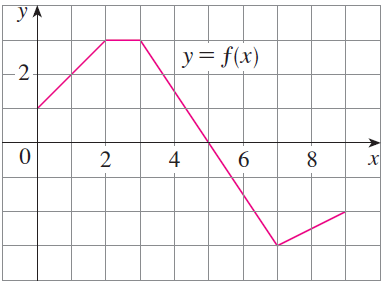
\includegraphics{5.2fig1}\\
			Evaluate each integral by interpreting it in terms of areas.
			\begin{enumerate}[(a)]
				\item \(\ds \int_0^2 f(x)\, dx\)
					\vs{1}
					
				\item \(\ds \int_0^5 f(x)\, dx\)
					\vs{1}
					
				\item \(\ds \int_5^7 f(x)\, dx\)
					\vs{1}
					
				\item \(\ds \int_0^9 f(x)\, dx\)
					\vs{1}
			\end{enumerate}
		\end{ex}
			\newpage
			
	\subsubsection*{Properties of the Definite Integral}
		The following are useful properties when working with the definite integral:
			\begin{thm}[Properties of the Definite Integral]
				 Let \(f,g\) be continuous functions on \([a,b]\).  Let \(c\) be a constant.  Then, \\
					\begin{enumerate}[(1)]
					\setlength\itemsep{35pt}
						\item 
						\item 
						\item 
						\item 
						\item 
						\item 
					\end{enumerate}
				
			\end{thm}
		
		\begin{ex}
			If \(\ds \int_0^6 f(x)\, dx = 10\) and \(\ds \int_0^8 f(x)\, dx = 4\), what is \(\ds\int_6^8 f(x)\, dx\)?
		\end{ex}	
			\vs{1.5}
			\newpage
	
		\begin{ex}
			Compute \(\ds \int_1^2 (4+2x^2)\,dx\).
		\end{ex}
			\vs{1}

		\begin{ex}
			For any \(a,b\), find the value of \(\ds \int_a^b x\, dx\) 			
		\end{ex}
			\vs{1}
			\newpage
			
		\begin{ex}
			Evaluate the integrals by interpreting them in terms of area:
			\begin{enumerate}[(a)]
				\item \(\ds \int_0^9 \lrpar{\dfrac{2}{3}x - 2}\, dx\)
					\vs{1}
					
				\item \(\ds \int_{-6}^6 \lrpar{x - \sqrt{36-x^2}}\, dx\)
					\vs{1}
					
				\item \(\ds \int_0^1 |2x - 1|\, dx\)
					\vs{1}
			\end{enumerate}
		\end{ex}
			\newpage 
		
	\subsection*{After Class Practice}
		\begin{ex}
			If \(\ds \int_0^9 f(x)\, dx = 37\) and \(\ds \int_0^9 g(x)\, dx = 16\), what is \(\ds \int_0^9 \lrpar{2f(x) + 3g(x)}\, dx\)?
		\end{ex}
			\vs{1}
		\begin{ex}
			If \(\ds \int_0^\pi \sin^4 x\, dx = \dfrac{3\pi}{8}\), what is \(\ds \int_\pi^0 \sin^4 x\, dx\)?  Why?
		\end{ex}
			\vs{1}
			\newpage
				
		\begin{ex}
			Use the definition of the integral to find \(\ds \int_1^4 \lrpar{x^2 - 4x + 2}\, dx \)
		\end{ex}
			\vs{2}
			
		
\clearpage
\end{document}
